\begin{frame}{Πειραματική διάταξη}

\definecolor{r}{RGB}{255 0 0}
\definecolor{g}{RGB}{0 155 0}

\begin{minipage}{\linewidth}
  \begin{minipage}{0.33\linewidth}
    \begin{figure}
      % GNUPLOT: LaTeX picture with Postscript
\begingroup
  \makeatletter
  \providecommand\color[2][]{%
    \GenericError{(gnuplot) \space\space\space\@spaces}{%
      Package color not loaded in conjunction with
      terminal option `colourtext'%
    }{See the gnuplot documentation for explanation.%
    }{Either use 'blacktext' in gnuplot or load the package
      color.sty in LaTeX.}%
    \renewcommand\color[2][]{}%
  }%
  \providecommand\includegraphics[2][]{%
    \GenericError{(gnuplot) \space\space\space\@spaces}{%
      Package graphicx or graphics not loaded%
    }{See the gnuplot documentation for explanation.%
    }{The gnuplot epslatex terminal needs graphicx.sty or graphics.sty.}%
    \renewcommand\includegraphics[2][]{}%
  }%
  \providecommand\rotatebox[2]{#2}%
  \@ifundefined{ifGPcolor}{%
    \newif\ifGPcolor
    \GPcolorfalse
  }{}%
  \@ifundefined{ifGPblacktext}{%
    \newif\ifGPblacktext
    \GPblacktexttrue
  }{}%
  % define a \g@addto@macro without @ in the name:
  \let\gplgaddtomacro\g@addto@macro
  % define empty templates for all commands taking text:
  \gdef\gplfronttext{}%
  \gdef\gplfronttext{}%
  \makeatother
  \ifGPblacktext
    % no textcolor at all
    \def\colorrgb#1{}%
    \def\colorgray#1{}%
  \else
    % gray or color?
    \ifGPcolor
      \def\colorrgb#1{\color[rgb]{#1}}%
      \def\colorgray#1{\color[gray]{#1}}%
      \expandafter\def\csname LTw\endcsname{\color{white}}%
      \expandafter\def\csname LTb\endcsname{\color{black}}%
      \expandafter\def\csname LTa\endcsname{\color{black}}%
      \expandafter\def\csname LT0\endcsname{\color[rgb]{1,0,0}}%
      \expandafter\def\csname LT1\endcsname{\color[rgb]{0,1,0}}%
      \expandafter\def\csname LT2\endcsname{\color[rgb]{0,0,1}}%
      \expandafter\def\csname LT3\endcsname{\color[rgb]{1,0,1}}%
      \expandafter\def\csname LT4\endcsname{\color[rgb]{0,1,1}}%
      \expandafter\def\csname LT5\endcsname{\color[rgb]{1,1,0}}%
      \expandafter\def\csname LT6\endcsname{\color[rgb]{0,0,0}}%
      \expandafter\def\csname LT7\endcsname{\color[rgb]{1,0.3,0}}%
      \expandafter\def\csname LT8\endcsname{\color[rgb]{0.5,0.5,0.5}}%
    \else
      % gray
      \def\colorrgb#1{\color{black}}%
      \def\colorgray#1{\color[gray]{#1}}%
      \expandafter\def\csname LTw\endcsname{\color{white}}%
      \expandafter\def\csname LTb\endcsname{\color{black}}%
      \expandafter\def\csname LTa\endcsname{\color{black}}%
      \expandafter\def\csname LT0\endcsname{\color{black}}%
      \expandafter\def\csname LT1\endcsname{\color{black}}%
      \expandafter\def\csname LT2\endcsname{\color{black}}%
      \expandafter\def\csname LT3\endcsname{\color{black}}%
      \expandafter\def\csname LT4\endcsname{\color{black}}%
      \expandafter\def\csname LT5\endcsname{\color{black}}%
      \expandafter\def\csname LT6\endcsname{\color{black}}%
      \expandafter\def\csname LT7\endcsname{\color{black}}%
      \expandafter\def\csname LT8\endcsname{\color{black}}%
    \fi
  \fi
  \setlength{\unitlength}{0.02500bp}%
  \begin{picture}(4000.00,4000.00)%
    \gplgaddtomacro\gplfronttext{%
      \colorrgb{0.00,0.00,0.00}%
      \put(388,778){\makebox(0,0)[r]{\strut{}\footnotesize $4$}}%
      \colorrgb{0.00,0.00,0.00}%
      \put(388,1295){\makebox(0,0)[r]{\strut{}\footnotesize $6$}}%
      \colorrgb{0.00,0.00,0.00}%
      \put(388,1811){\makebox(0,0)[r]{\strut{}\footnotesize $8$}}%
      \colorrgb{0.00,0.00,0.00}%
      \put(388,2328){\makebox(0,0)[r]{\strut{}\footnotesize $10$}}%
      \colorrgb{0.00,0.00,0.00}%
      \put(388,2844){\makebox(0,0)[r]{\strut{}\footnotesize $12$}}%
      \colorrgb{0.00,0.00,0.00}%
      \put(388,3361){\makebox(0,0)[r]{\strut{}\footnotesize $14$}}%
      \colorrgb{0.00,0.00,0.00}%
      \put(778,300){\makebox(0,0){\strut{}\footnotesize $4$}}%
      \colorrgb{0.00,0.00,0.00}%
      \put(1295,300){\makebox(0,0){\strut{}\footnotesize $6$}}%
      \colorrgb{0.00,0.00,0.00}%
      \put(1811,300){\makebox(0,0){\strut{}\footnotesize $8$}}%
      \colorrgb{0.00,0.00,0.00}%
      \put(2328,300){\makebox(0,0){\strut{}\footnotesize $10$}}%
      \colorrgb{0.00,0.00,0.00}%
      \put(2844,300){\makebox(0,0){\strut{}\footnotesize $12$}}%
      \colorrgb{0.00,0.00,0.00}%
      \put(3361,300){\makebox(0,0){\strut{}\footnotesize $14$}}%
      \colorrgb{0.00,0.00,0.00}%
      \put(-318,2069){\rotatebox{90}{\makebox(0,0){\strut{}$y$ [m]}}}%
      \colorrgb{0.00,0.00,0.00}%
      \put(2069,-230){\makebox(0,0){\strut{}$x$ [m]}}%
    }%
    \gplgaddtomacro\gplfronttext{%
    }%
    \put(0,0){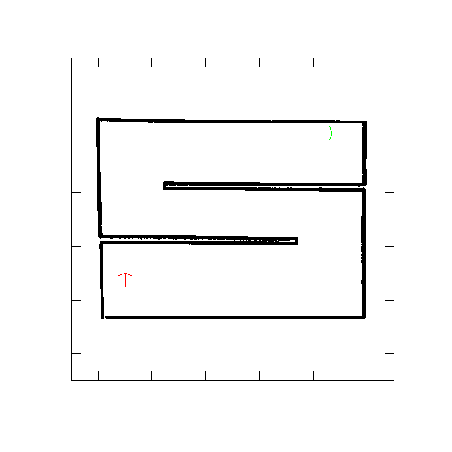
\includegraphics[scale=0.5]{./figures/slides/ch3/corridor}}%
    \gplfronttext
  \end{picture}%
\endgroup

      \vspace{0.15cm}
      \caption{\tiny Χάρτης περιβάλλοντος CORRIDOR, $\bm{M}_C$}
    \end{figure}
  \end{minipage}
  \begin{minipage}{0.33\linewidth}
    \begin{figure}
      \definecolor{r}{RGB}{255 0 0}
\definecolor{g}{RGB}{0 155 0}
% GNUPLOT: LaTeX picture with Postscript
\begingroup
  \makeatletter
  \providecommand\color[2][]{%
    \GenericError{(gnuplot) \space\space\space\@spaces}{%
      Package color not loaded in conjunction with
      terminal option `colourtext'%
    }{See the gnuplot documentation for explanation.%
    }{Either use 'blacktext' in gnuplot or load the package
      color.sty in LaTeX.}%
    \renewcommand\color[2][]{}%
  }%
  \providecommand\includegraphics[2][]{%
    \GenericError{(gnuplot) \space\space\space\@spaces}{%
      Package graphicx or graphics not loaded%
    }{See the gnuplot documentation for explanation.%
    }{The gnuplot epslatex terminal needs graphicx.sty or graphics.sty.}%
    \renewcommand\includegraphics[2][]{}%
  }%
  \providecommand\rotatebox[2]{#2}%
  \@ifundefined{ifGPcolor}{%
    \newif\ifGPcolor
    \GPcolorfalse
  }{}%
  \@ifundefined{ifGPblacktext}{%
    \newif\ifGPblacktext
    \GPblacktexttrue
  }{}%
  % define a \g@addto@macro without @ in the name:
  \let\gplgaddtomacro\g@addto@macro
  % define empty templates for all commands taking text:
  \gdef\gplfronttext{}%
  \gdef\gplfronttext{}%
  \makeatother
  \ifGPblacktext
    % no textcolor at all
    \def\colorrgb#1{}%
    \def\colorgray#1{}%
  \else
    % gray or color?
    \ifGPcolor
      \def\colorrgb#1{\color[rgb]{#1}}%
      \def\colorgray#1{\color[gray]{#1}}%
      \expandafter\def\csname LTw\endcsname{\color{white}}%
      \expandafter\def\csname LTb\endcsname{\color{black}}%
      \expandafter\def\csname LTa\endcsname{\color{black}}%
      \expandafter\def\csname LT0\endcsname{\color[rgb]{1,0,0}}%
      \expandafter\def\csname LT1\endcsname{\color[rgb]{0,1,0}}%
      \expandafter\def\csname LT2\endcsname{\color[rgb]{0,0,1}}%
      \expandafter\def\csname LT3\endcsname{\color[rgb]{1,0,1}}%
      \expandafter\def\csname LT4\endcsname{\color[rgb]{0,1,1}}%
      \expandafter\def\csname LT5\endcsname{\color[rgb]{1,1,0}}%
      \expandafter\def\csname LT6\endcsname{\color[rgb]{0,0,0}}%
      \expandafter\def\csname LT7\endcsname{\color[rgb]{1,0.3,0}}%
      \expandafter\def\csname LT8\endcsname{\color[rgb]{0.5,0.5,0.5}}%
    \else
      % gray
      \def\colorrgb#1{\color{black}}%
      \def\colorgray#1{\color[gray]{#1}}%
      \expandafter\def\csname LTw\endcsname{\color{white}}%
      \expandafter\def\csname LTb\endcsname{\color{black}}%
      \expandafter\def\csname LTa\endcsname{\color{black}}%
      \expandafter\def\csname LT0\endcsname{\color{black}}%
      \expandafter\def\csname LT1\endcsname{\color{black}}%
      \expandafter\def\csname LT2\endcsname{\color{black}}%
      \expandafter\def\csname LT3\endcsname{\color{black}}%
      \expandafter\def\csname LT4\endcsname{\color{black}}%
      \expandafter\def\csname LT5\endcsname{\color{black}}%
      \expandafter\def\csname LT6\endcsname{\color{black}}%
      \expandafter\def\csname LT7\endcsname{\color{black}}%
      \expandafter\def\csname LT8\endcsname{\color{black}}%
    \fi
  \fi
  \setlength{\unitlength}{0.03200bp}%
  \begin{picture}(4000.00,5000.00)%
    \gplgaddtomacro\gplfronttext{%
      \colorrgb{0.00,0.00,0.00}%
      \put(520,727){\makebox(0,0)[r]{\strut{} \footnotesize $0$}}%
      \colorrgb{0.00,0.00,0.00}%
      \put(520,1170){\makebox(0,0)[r]{\strut{}\footnotesize $5$}}%
      \colorrgb{0.00,0.00,0.00}%
      \put(520,1613){\makebox(0,0)[r]{\strut{}\footnotesize $10$}}%
      \colorrgb{0.00,0.00,0.00}%
      \put(520,2056){\makebox(0,0)[r]{\strut{}\footnotesize $15$}}%
      \colorrgb{0.00,0.00,0.00}%
      \put(520,2498){\makebox(0,0)[r]{\strut{}\footnotesize $20$}}%
      \colorrgb{0.00,0.00,0.00}%
      \put(520,2941){\makebox(0,0)[r]{\strut{}\footnotesize $25$}}%
      \colorrgb{0.00,0.00,0.00}%
      \put(520,3384){\makebox(0,0)[r]{\strut{}\footnotesize $30$}}%
      \colorrgb{0.00,0.00,0.00}%
      \put(520,3827){\makebox(0,0)[r]{\strut{}\footnotesize $35$}}%
      \colorrgb{0.00,0.00,0.00}%
      \put(520,4270){\makebox(0,0)[r]{\strut{}\footnotesize $40$}}%
      \colorrgb{0.00,0.00,0.00}%
      \put(1095,330){\makebox(0,0){\strut{}\footnotesize $0$}}%
      \colorrgb{0.00,0.00,0.00}%
      \put(1538,330){\makebox(0,0){\strut{}\footnotesize $5$}}%
      \colorrgb{0.00,0.00,0.00}%
      \put(1980,330){\makebox(0,0){\strut{}\footnotesize $10$}}%
      \colorrgb{0.00,0.00,0.00}%
      \put(2423,330){\makebox(0,0){\strut{}\footnotesize $15$}}%
      \colorrgb{0.00,0.00,0.00}%
      \put(2866,330){\makebox(0,0){\strut{}\footnotesize $20$}}%
      \colorrgb{0.00,0.00,0.00}%
      \put(-94,2587){\rotatebox{90}{\makebox(0,0){\strut{}$y$ [m]}}}%
      \colorrgb{0.00,0.00,0.00}%
      \put(2069,0){\makebox(0,0){\strut{}$x$ [m]}}%
      \put(2750,1300){\makebox(0,0){\strut{}\textcolor{g}{$\bm{p}_0$}}}%
      \put(2000,4300){\makebox(0,0){\strut{}\textcolor{r}{$\bm{p}_G$}}}%
    }%
    \gplgaddtomacro\gplfronttext{%
    }%
    \put(0,0){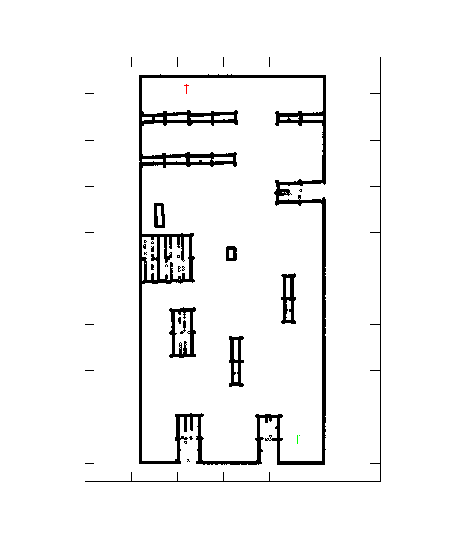
\includegraphics[scale=0.64]{./figures/slides/ch4/warehouse}}%
    \gplfronttext
  \end{picture}%
\endgroup

      \vspace{0.15cm}
      \caption{\tiny Χάρτης περιβάλλοντος WAREHOUSE, $\bm{M}_W$}
    \end{figure}
  \end{minipage}
  \begin{minipage}{0.3\linewidth}
    $N = 100 \times $ $\textcolor{g}{\bm{p}_0} \rightarrow \textcolor{r}{\bm{p}_G}$\\

    lidar:

    $\lambda = 260^\circ$

    $N_s = 640$ ακτίνες

    {\footnotesize $W_R \sim \mathcal{N}(0,\sigma_R^2=0.01^2)$ $[$m, m$^2]$} \\

    \texttt{pf}:

    $200 \leq |\mathcal{P}| \leq 500$

  \end{minipage}

\end{minipage}


\note{\footnotesize
Για να δοκιμάσουμε τις τρεις υποθέσεις χρησιμοποιούμε δύο περιβάλλοντα, ένα
  απλό, και ένα που ομοιάζει σε αποθήκη, δηλαδή το αναμενόμενο περιβάλλον των
  ρομπότ που κατασκευάσαμε για το έργο RELIEF. Για κάθε περίπτωση διαλογής
  σωματιδίων και μεθόδου ανάδρασης από το ρομπότ ζητήθηκε να πλοηγηθεί αυτόνομα
  από μία αρχική σε μία τελική στάση 100 διαφορετικές φορές. Το ρομπότ φέρει
  έναν αισθητήρα lidar γωνιακού εύρους 260 μοιρών, με θόρυβο
  μέτρησης κανονικά κατανεμημένο με τυπική απόκλιση ενός εκατοστού. Ο πληθυσμός
  του φίλτρου είναι κυμαινόμενος με ελάχιστη πληθικότητα 200 σωματίδια, και
  μέγιστη 500.}


\end{frame}
